\documentclass[12pt]{article}

\usepackage[utf8]{inputenc}
\usepackage{amsmath}
\usepackage{graphicx}
\usepackage{titlesec}
\usepackage{tcolorbox}
\usepackage{titling}
\usepackage{circuitikz}
\usepackage{enumitem}
\usepackage{wrapfig}
\usepackage{float}
\usepackage{pgfplots}
\usepackage{hyperref}
\pgfplotsset{compat=1.18}

\title{\bfseries Laborator Electricitate 3}
\author{Sîrghe Matei}
\date{\today}

\pretitle{\begin{center}\LARGE\bfseries}
\posttitle{\par\end{center}\vskip 0.5em}
\preauthor{\begin{center}\large}
\postauthor{\end{center}}
\predate{\begin{center}\large}
\postdate{\end{center}}

\titleformat{\section}
  {\normalfont\Large\bfseries}{\thesection}{1em}{}

\begin{document}

\maketitle

\begin{center}
    \LARGE\textit{Studiul condensatorului electric cu fețe plan-paralele și}
    \LARGE\textit{Determinarea constantei dielectrice a unui izolator}
\end{center}

\section{Teoria Lucrării}

\subsection{Schema Electrică}

\begin{minipage}{0.45\textwidth}
    \centering
    \textbf{Notație condensator :}
    \begin{circuitikz} \draw
        (0,0) to[C] (2,0);
    \end{circuitikz}
\end{minipage}
\hfill
\begin{minipage}{0.45\textwidth}
    \centering
    \begin{circuitikz} \draw
        (0,0) to[ground] (0,-0.2) node[ground] {}
        (0,0) to[battery] (2,0)
        to[C] (4,0)
        to[ground] (5,0) node[ground] {};
        \draw (2,1) node[right] {$+Q$};
        \draw (3,1) node[right] {$-Q$};
        \draw (2,-1) node[right] {$5C$};
        \draw (3,-1) node[right] {$-5C$};
    \end{circuitikz}
\end{minipage}


\noindent
\textbf{Definiție : }Condensatorul electric este un dispozitiv format din doua plăci metalice așezate față în față separate de un mediu izolator sau dielectric.
Plăcile metalice ale condensatorului se numesc armături și se încarcă cu aceeași cantitate de sarcină electrică dar de semn opus. Proprietatea
fundamentală a unui condensator electric este aceea de a înmagazina $($reține$)$ pentru un anumit interval de timp sarcină electrică.

\noindent
\textbf{Mărimi fizice :} $[C]_{SI}$ Mărimea fizică care descrie comportamentele unui condensator electric se numește
capacitate electrică și în sistemul internațional de unități se măsoară în \textbf{Farad}.

\begin{center}
    \centering
    \begin{circuitikz} \draw
        (0,0) to[ground] (0,-0.2) node[ground] {}
        (0,0) to[battery] (2,0)
        to[C] (4,0)
        to[ground] (5,0) node[ground] {};
        \draw (2,1) node[right] {$+Q$};
        \draw (3,1) node[right] {$-Q$};
        \draw (2,-1) node[right] {$\varphi_{N}$};
        \draw (3,-1) node[right] {$\varphi_{M}=0$};
    \end{circuitikz}
\end{center}

\noindent
\textbf{Formule fizice :}
\begin{enumerate}
    \item $[C]_{SI}$ = 1 F (Farad) = 1 C/V (Coulomb pe Volt)
    \item $C=\frac{+Q}{\varphi_{N}-\varphi_{M}}=\frac{-Q}{\varphi_{M}-\varphi_{N}}=\frac{\left| Q \right|}{U_{NM}}$
    \item $\Delta\varphi = U $ - tensiune electrică
    \item $\left| \varphi_{M}-\varphi_{N} \right| = U_{NM} $ - Diferența de potențial 
\end{enumerate}

\subsection{Montajul Experimental}

\begin{center}
    \centering
    \begin{circuitikz} \draw
        (0,0) to[ground] (0,-2) node[ground] {}
        (0,0) to[battery] (2,0)
        to[C] (5,0)
        (5,0)to[ground] (5,-2) node[ground] {}
        (5,0) to[C] (6,0)
        
        (8,0) node[op amp] (opamp) {};
        \draw (opamp.+) -- ++(0,-0.5) -| (5,0) {};
        \draw (opamp.-) -- ++(0,0) -| (6,0);
        \draw (opamp.out)(9,0) to[voltmeter] (10,0) node[right] {Out};

        \draw (0,-1) node[right] {$[\varphi]=V$};
        \draw (0,1) node[right] {$+$};
        \draw (2.5,0.5) node[right] {$+Q$};
        \draw (3.5,0.5) node[right] {$-Q$};
        \draw (3.25,-0.75) node[right] {$C$};
        \draw (5.25,-0.75) node[right] {$C_{0}$};
    \end{circuitikz}
\end{center}

\subsection{Determinarea capacității electrice necunoscute C}
Valoarea lui C va fi determinată prin metoda grafică.\\

$C=\frac{Q}{\varphi}$ \hspace{2cm} $C_{0}=\frac{Q}{U}$ \hspace{2cm}  $Q=C_{0}U \hspace{2cm}  C=\frac{C_{0}*U}{\varphi}$\\

$\varphi- $ Este modificat \hspace{2cm} $U- $Date primare\\

\begin{tcolorbox}[colback=yellow!10!white, colframe=black, title=Observație]
Teoria discutată la acest punct al experimentului este validă dacă și numai dată distanța dintre cele două armături (d) este constantă.
\end{tcolorbox}

\subsection{Verificarea legii C \textasciitilde $\frac{1}{d}$}
Distanța dintre armături va fi modificată astfel încât să putem verifica legea C \textasciitilde $\frac{1}{d}$.\\

$C=\frac{Q}{\varphi}$ \hspace{2cm} $C_{0}=\frac{Q}{U}$ \hspace{2cm}  $Q=C_{0}U \hspace{2cm}  C=\frac{C_{0}*U}{\varphi}$\\

$d- $ Este modificat \hspace{2cm} $C- $Calculat de noi\\

\begin{tcolorbox}[colback=yellow!10!white, colframe=black, title=Observație]
Teoria discutată pentru acest subpunct al experimentului este validă dacă și numai dacp diferența de potențial aplicată cu ajutorul
sursei de înaltă tensiune rămâne constantă. ($\varphi- $ cnst.)
\end{tcolorbox}

\subsection{ Determinarea constantei dielectrice a unui izolator \textbf{$(\epsilon_{r})$}}

\begin{wrapfigure}{r}{0.3\textwidth} 
    \centering
    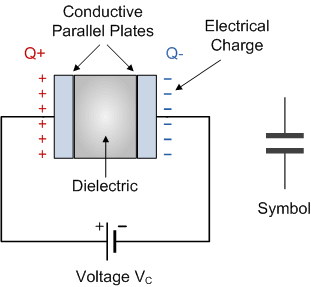
\includegraphics[width=0.38\textwidth]{dielectric.png} 
    \caption{Izolator dielectric}
    \label{fig:Dielectric}
\end{wrapfigure}

Pentru punctele a) și b) izolatorul considerat a fost aer. Pentru acest punct, vom face mai întâi determinări experimentale folosind aerul
ca izolator iar apoi în același condiții experimentale vom face măsurători folosind o placă de plastic pe care o vom introduce între cele două armături.\\

$\varphi$ = constant ; d=constant \\

$C_{aer}=\frac{Q_{aer}}{\varphi_{aer}}$  ;  $C_{0}=\frac{Q_{aer}}{U_{aer}}$\\

$C_{aer}=\frac{C_{0}*U_{aer}}{\varphi}$  ; $\varphi_{aer}=\varphi$\\

$C_{izolator}=\frac{Q_{izolator}}{\varphi}=\frac{C_{0}*U_{izolator}}{\varphi}$\\

$\epsilon_{r}=\frac{C_{izolator}}{C_{aer}}$  ;  $\epsilon_{r}-adimensional$\\



\section{Datele Experimentului Primare}
Acestea sunt datele exerimentale : 

\subsection{Tabel pentru subpunctul A}

\begin{table}[h!]
    \centering
    \begin{tabular}{|c|c|c|c|}
        \hline
        Nr. Experiment & $\varphi (kV)$ & $U (V)$  & $d (cm)$ \\
        \hline
        1 & 1,1 & 0,32 & 0,5 \\
        \hline
        2 & 1,4 & 0,42 & 0,5 \\
        \hline
        3 & 1,7 & 0,52 & 0,5 \\
        \hline
        4 & 2,0 & 0,62 & 0,5 \\
        \hline
        5 & 2,3 & 0,72 & 0,5 \\
        \hline
        6 & 2,6 & 0,80 & 0,5 \\
        \hline
        7 & 2,9 & 0,86 & 0,5 \\
        \hline
        8 & 3,2 & 0,98 & 0,5 \\
        \hline
    \end{tabular}
\end{table}

\subsection{Tabel pentru subpunctul B}

\begin{table}[h!]
    \centering
    \begin{tabular}{|c|c|c|c|}
        \hline
        Nr. Experiment & $\varphi (kV)$ & $U (V)$  & $d (cm)$ \\
        \hline
        1 & 2,0 & 1,00 & 0,5 \\
        \hline
        2 & 2,0 & 0,80 & 0,8 \\
        \hline
        3 & 2,0 & 0,56 & 1,1 \\
        \hline
        4 & 2,0 & 0,48 & 1,4 \\
        \hline
        5 & 2,0 & 0,44 & 1,7 \\
        \hline
        6 & 2,0 & 0,40 & 2,0 \\
        \hline
        7 & 2,0 & 0,38 & 2,1 \\
        \hline
    \end{tabular}
\end{table}

\subsection{Tabel pentru subpunctul C}

\begin{table}[H]
    \centering
    \begin{tabular}{|c|c|c|c|c|}
        \hline
        Nr. Experiment & $\varphi (kV)$ & $U (V)$  & $d (cm)$ & izolator \\
        \hline
        1 & 5,0 & 2,80 & 1 & plastic \\
        \hline
        2 & 5,0 & 1,30 & 1 & aer \\
        \hline
        3 & 2,5 & 2,00 & 1 & plastic \\
        \hline
        4 & 2,5 & 0,74 & 1 & aer\\
        \hline
    \end{tabular}
\end{table}

\section{Prelucrarea datelor experimentale}

\subsection{Calcule punctul A}

$Q_{1} = C_{0}U=0,22 \times 10^{-6}F \times 0,32V = 7 \times 10^{-8}C = 0,7 \times 10^{-7}C $\\
$Q_{2} = C_{0}U=0,22 \times 10^{-6}F \times 0,42V = 9 \times 10^{-8}C = 0,9 \times 10^{-7}C $\\
$Q_{3} = C_{0}U=0,22 \times 10^{-6}F \times 0,52V = 1,1 \times 10^{-7}C$\\
$Q_{4} = C_{0}U=0,22 \times 10^{-6}F \times 0,62V = 1,3 \times 10^{-7}C$\\
$Q_{5} = C_{0}U=0,22 \times 10^{-6}F \times 0,72V = 1,5 \times 10^{-7}C$\\
$Q_{6} = C_{0}U=0,22 \times 10^{-6}F \times 0,80V = 1,7 \times 10^{-7}C$\\
$Q_{7} = C_{0}U=0,22 \times 10^{-6}F \times 0,86V = 1,9 \times 10^{-7}C$\\
$Q_{8} = C_{0}U=0,22 \times 10^{-6}F \times 0,98V = 2,1 \times 10^{-7}C$\\

\begin{figure}[H]
    \centering
    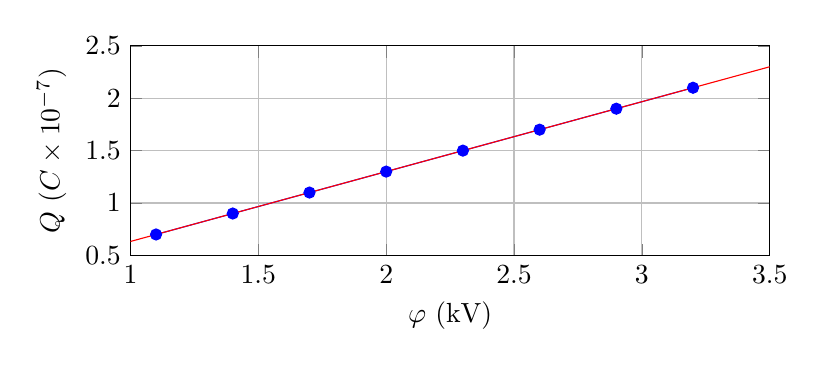
\begin{tikzpicture}
        \begin{axis}[
            xlabel={$\varphi$ (kV)},
            ylabel={$Q$ ($C \times 10^{-7}$)},
            grid=major,
            width=0.8\textwidth,
            height=0.35\textwidth,
            xmin=1, xmax=3.5,
            ymin=0.5, ymax=2.5,
        ]
        \addplot[
            color=blue,
            mark=*,
            ]
            coordinates {
                (1.1, 0.7)
                (1.4, 0.9)
                (1.7, 1.1)
                (2.0, 1.3)
                (2.3, 1.5)
                (2.6, 1.7)
                (2.9, 1.9)
                (3.2, 2.1)
            };
        \addplot [
            domain=1:3.5, 
            samples=100, 
            color=red,
        ]{0.6667*x -0.03333};
        \end{axis}
    \end{tikzpicture}
    \caption{Grafic cu $Q$ și $\varphi$}
    \label{fig:Q_vs_rho}
\end{figure}

Am utilizat site-ul \href{https://www.graphpad.com}{GraphPad} pentru a obține dreapta de regresie liniară.Ecuația obținută este : $Q=0,6667 \times \varphi-0,03333 \implies C=0,6667 \times 10^{-7}F$\\

\subsection{Calcule punctul B}
$Q_{1} = C_{0}U = 0,22 \times 10^{-6}F \times 1,00V = 2,2 \times 10^{-7}C$\\
$C_{1} = \frac{Q_{1}}{\varphi} = \frac{2,2 \times 10^{-7}C}{2,0kV} = 1,1 \times 10^{-7}F$\\
$Q_{2} = C_{0}U = 0,22 \times 10^{-6}F \times 0,80V = 1,76 \times 10^{-7}C$\\
$C_{2} = \frac{Q_{2}}{\varphi} = \frac{1,76 \times 10^{-7}C}{2,0kV} = 0,88 \times 10^{-7}F$\\
$Q_{3} = C_{0}U = 0,22 \times 10^{-6}F \times 0,56V = 1,232 \times 10^{-7}C$\\
$C_{3} = \frac{Q_{3}}{\varphi} = \frac{1,232 \times 10^{-7}C}{2,0kV} = 0,616 \times 10^{-7}F$\\
$Q_{4} = C_{0}U = 0,22 \times 10^{-6}F \times 0,48V = 1,056 \times 10^{-7}C$\\
$C_{4} = \frac{Q_{4}}{\varphi} = \frac{1,056 \times 10^{-7}C}{2,0kV} = 0,528 \times 10^{-7}F$\\
$Q_{5} = C_{0}U = 0,22 \times 10^{-6}F \times 0,44V = 0,968 \times 10^{-7}C$\\
$C_{5} = \frac{Q_{5}}{\varphi} = \frac{0,968 \times 10^{-7}C}{2,0kV} = 0,484 \times 10^{-7}F$\\
$Q_{6} = C_{0}U = 0,22 \times 10^{-6}F \times 0,40V = 0,88 \times 10^{-7}C$\\
$C_{6} = \frac{Q_{6}}{\varphi} = \frac{0,88 \times 10^{-7}C}{2,0kV} = 0,44 \times 10^{-7}F$\\
$Q_{7} = C_{0}U = 0,22 \times 10^{-6}F \times 0,38V = 0,836 \times 10^{-7}C$\\
$C_{7} = \frac{Q_{7}}{\varphi} = \frac{0,836 \times 10^{-7}C}{2,0kV} = 0,418 \times 10^{-7}F$\\

\begin{figure}[H]
    \centering
    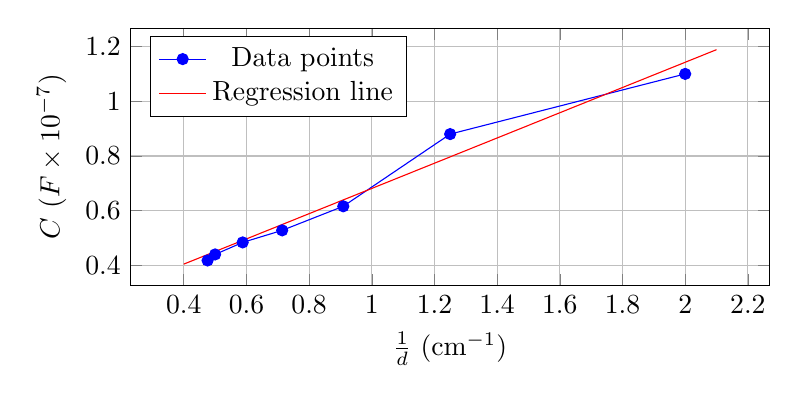
\begin{tikzpicture}
        \begin{axis}[
            xlabel={$\frac{1}{d}$ (cm$^{-1}$)},
            ylabel={$C$ ($F \times 10^{-7}$)},
            grid=major,
            width=0.8\textwidth,
            height=0.4\textwidth,
            legend pos=north west,
        ]
        \addplot[
            color=blue,
            mark=*,
            ]
            coordinates {
                (2.0, 1.1)
                (1.25, 0.88)
                (0.909, 0.616)
                (0.714, 0.528)
                (0.588, 0.484)
                (0.5, 0.44)
                (0.476, 0.418)
            };
        \addlegendentry{Data points}

        \addplot [
            domain=0.4:2.1, 
            samples=100, 
            color=red,
        ]{0.4613*x +0.22 };
        \addlegendentry{Regression line}
        \end{axis}
    \end{tikzpicture}
    \caption{Grafic cu $C$ și $\frac{1}{d}$}
    \label{fig:C_vs_1_d}
\end{figure}

Am utilizat site-ul \href{https://www.graphpad.com}{GraphPad} pentru a obține dreapta de regresie liniară. Ecuația obținută este : $f = 0.4613 \times x + 0.22 \implies$ Din pantă și calculele făcute : 2 $\times C \approx \frac{1}{d}$\\

\subsection{Calcule punctul C}
\begin{equation}
C_{0} = 0.22 \times 10^{-6} \, F
\end{equation}
\begin{equation}
Q_{1,\text{plastic}} = C_{0}U = 0.22 \times 10^{-6}F \times 2.80V = 6.16 \times 10^{-7}C\\
\end{equation}
\begin{equation}
C_{1,\text{plastic}} = \frac{Q_{1,\text{plastic}}}{\varphi} = \frac{6.16 \times 10^{-7}C}{5.0kV} = 1.232 \times 10^{-7}F\\
\end{equation}
\begin{equation}
Q_{1,\text{aer}} = C_{0}U = 0.22 \times 10^{-6}F \times 1.30V = 2.86 \times 10^{-7}C\\
\end{equation}
\begin{equation}
C_{1,\text{aer}} = \frac{Q_{1,\text{aer}}}{\varphi} = \frac{2.86 \times 10^{-7}C}{5.0kV} = 0.572 \times 10^{-7}F\\
\end{equation}
\begin{equation}
\epsilon_{r1} = \frac{C_{1,\text{plastic}}}{C_{1,\text{aer}}} = \frac{1.232 \times 10^{-7}F}{0.572 \times 10^{-7}F} \approx 2.15\\
\end{equation}
\begin{equation}
Q_{2,\text{plastic}} = C_{0}U = 0.22 \times 10^{-6}F \times 2.00V = 4.4 \times 10^{-7}C\\
\end{equation}
\begin{equation}
C_{2,\text{plastic}} = \frac{Q_{2,\text{plastic}}}{\varphi} = \frac{4.4 \times 10^{-7}C}{2.5kV} = 1.76 \times 10^{-7}F\\
\end{equation}
\begin{equation}
Q_{2,\text{aer}} = C_{0}U = 0.22 \times 10^{-6}F \times 0.74V = 1.628 \times 10^{-7}C\\
\end{equation}
\begin{equation}
C_{2,\text{aer}} = \frac{Q_{2,\text{aer}}}{\varphi} = \frac{1.628 \times 10^{-7}C}{2.5kV} = 0.6512 \times 10^{-7}F\\
\end{equation}
\begin{equation}
\epsilon_{r2} = \frac{C_{2,\text{plastic}}}{C_{2,\text{aer}}} = \frac{1.76 \times 10^{-7}F}{0.6512 \times 10^{-7}F} \approx 2.70\\
\end{equation}

\section{Concluzii}

În urma experimentelor, am demonstrat că \( C \sim \frac{1}{d} \), am calculat valorile capacităților electrice pentru diferite distanțe și am determinat constantele dielectrice ale izolatorilor folosiți, obținând valori de aproximativ 2.15 și 2.70 pentru plastic.

\end{document}